\section{Introduction}
In the previous chapters, 
onemax function, 1D and 2D Ising models are employed 
for the benchmark problems.
The difference among the three problems is 
the number of correlations, 
which has an effect on the complexity of the cost function and 
the target distributions.
However, there are some different types of the difficulty of
optimization problems.
Hence, the objective of this chapter is
to conduct experiments to reveal the comprehensive effectiveness and 
property of RPM and HIS by using different types of problems.

In the following,
first, this chapter approaches 
towards the problems of 2D Ising with frustration.
The frustration of 2D Ising has an effect of instability, 
which means increasing the number of solutions
which have the same cost function value. 

Second,
this chapter approaches towards continuous problems.
Continuous problems seems to be more difficult than discrete problems.
In Ising models, undetected correlations are the difficulty.
In continuous space, additionally, the complexity of each dimension 
can have an effect on the difficulty.


\section{Advanced Benchmark Problems}
\subsection{Frustration}
\subsubsection{2D Ising model with Frustration}
In 1D or 2D Ising models,
the connections, which are defined by $J(x_i,x_j)$ 
in (\ref{ising-connection}), 
can be seen as constraints and
the cost function value represents the number of satisfied connections.
The frustration means existing unsatisfied constraints in any solutions.
This situation can be easily realized by
changing a part of connections $J(x_i,x_j)$ to
\begin{equation}
 J^{-}(x_i,x_j)= \left\{
  \begin{array}{rl}
    0 & x_i=x_j \\
    1 & x_i \neq x_j
  \end{array} \right.
.
\end{equation}

In 2D Ising models without frustration,
the optimum cost function value is given by
$-2d$, where $d$ is the number of the dimensions.
If just one connection is changed to be $J^{-}$
the cost function value of the optimum solution
becomes $-2d+1$.
Hence, if just $k\% \, (k<50)$ connections are changed to be $J^{-}$
and they are independent,
the cost function value of the optimum solution
can become $-2d(100-k)/100$.
However, if there exists some regularities, for example,
horizontal connections are $J$ and vertical connections are $J^{-}$,
the cost function value of the optimum solution
becomes $\{-2d(100-k)/100\}-\alpha$,
where $\alpha$ is an improvement term and its value is difficult to calculate in general.



\subsection{Continuous Problems}
This section introduces two continuous problems.

\subsubsection{Rosenbrock Function}
Rosenbrock Function\cite{shang:rosen} is defined as follows:
\begin{equation}
 f(x)= \sum_{i=1}^{d-1} (100 (x_i^2-x_{i+1})^2+(x_i-1)^2).
\end{equation}
If the second term is ignored,
the condition of $f'(x)=0$ is $x_i^2=x_{i+1}$.
This feature is shown in Fig. \ref{fig-rosenbrock}
The property of this problem is ill-scaled,
which means each dimension is correlated to each other.
This function can be seen almost as unimodal, which means that there is no
local optima. 
%cite{rosen}


\subsubsection{Rastrigin Function}
Rastrigin Function is defined as follows:
\begin{equation}
 f(x)=10d+\sum_{i=1}^d \{ x_i^2 - 10 \cos(2\pi x_i)\}.
\end{equation}
The feature is that
there are many local optima as shown in Fig. \ref{fig-rastrigin}
and,
therefore, this is quite hard problem for gradient-based methods.
There is no correlation.

\begin{figure}[tbp]
\centerline{
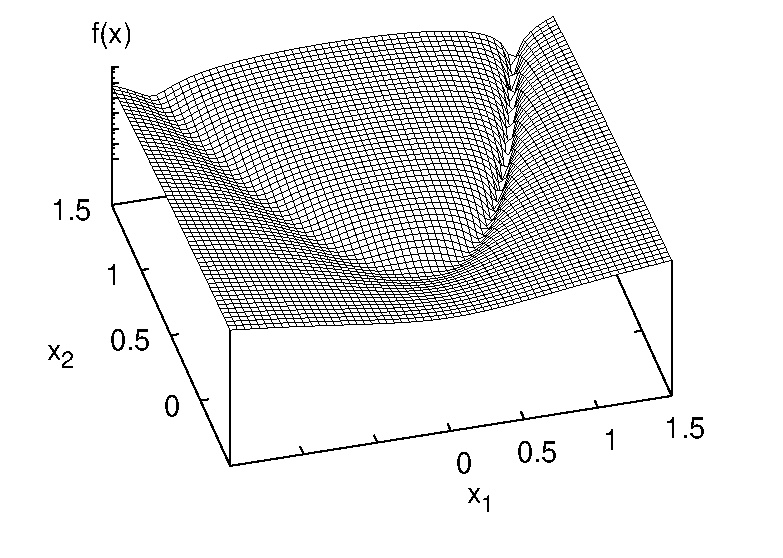
\includegraphics[width=\figlength\linewidth]{./data_aexp/rosenbrock.eps}}
\caption{2D Rosenbrock Function}
\label{fig-rosenbrock}

\vspace{\figskiplength}

\centerline{
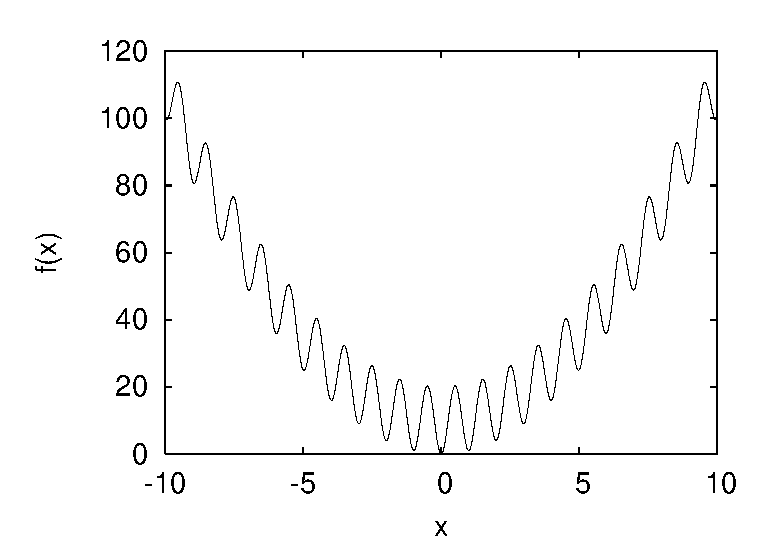
\includegraphics[width=\figlength\linewidth]{./data_aexp/rastrigin.eps}}
\caption{1D Rastrigin Function}
\label{fig-rastrigin}
\end{figure}


\section{Experiments on Frustration}
\subsection{Experimental Setup}
Three problems are employed.
One is a normal 2D Ising model.
For the others, $5\%$ are $10\%$ of the conncetions
are changed to $J^-$, respectively.
The number of the dimension is $400$.

EDA, RPM and HIS are compared.
Their parameters are determined as follows:
\begin{itemize}
 \item EDA
       \begin{itemize}
	\item $N$: $100$, $500$, $1000$, $3000$, or $6000$.
	\item $c$: $0.1$, $0.3$, or $0.5$.
       \end{itemize}
 \item RPM
       \begin{itemize}
	\item $N$: $10$, $50$, $100$, $200$, $300$, $400$, or $500$.
	\item $M(\leq N)$: $10$, $50$, $100$, $200$, $300$, $400$, or $500$.
	\item $c$: $0.01$ or $0.05$
       \end{itemize}
 \item HIS
       \begin{itemize}
	\item $M$: $10$
	\item $L$: $30$
       \end{itemize}
\end{itemize}
The setting of the probability models is the same as the previous chapters.
For each setting, we perform ten independent runs.


\subsection{Results}
The results are shown in Figs. \ref{result-2d-flust0},
\ref{result-2d-flust5}, and 
\ref{result-2d-flust10}.
The horizontal axis represents the number of function evaluations
performed and
the vertical axis represents the cost function value of the best
obtained solution.
Additionally, the horizontal lines in Figs.
\ref{result-2d-flust5} and 
\ref{result-2d-flust10}
show
the estimated optimal cost function values given by
$-2 \times d \times (1-p(J^-))$. 

The results show that the frustration cases have no serious problem 
since the estimated optimal values are almost obtained.
However, in 2D Ising model with changing $10\%$ connections,
the difference between
the cost function value of the obtained solutions of RPM and HIS
becomes smaller than the others.

\begin{figure}[tbp]
\centerline{
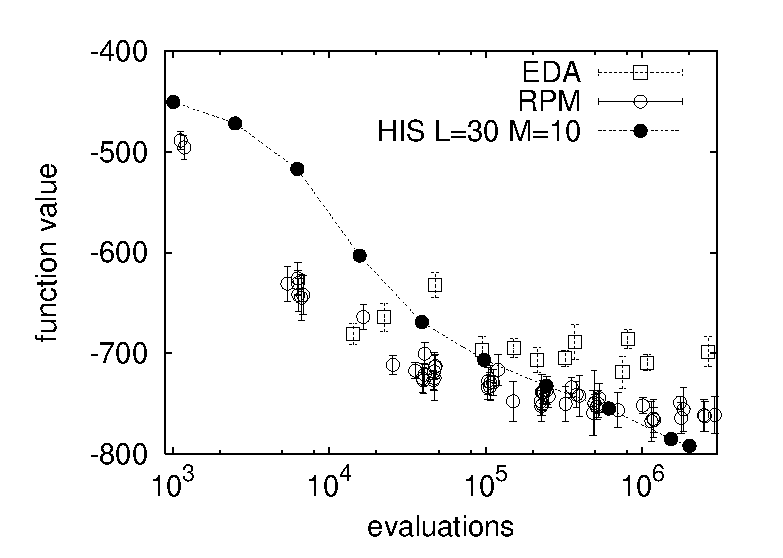
\includegraphics[width=\figlength\linewidth]{./data_aexp/2d_100.eps}}
\caption{2D Ising with $p(J^{-})=0$.}
\label{result-2d-flust0}
\end{figure}
\begin{figure}[tbp]
\centerline{
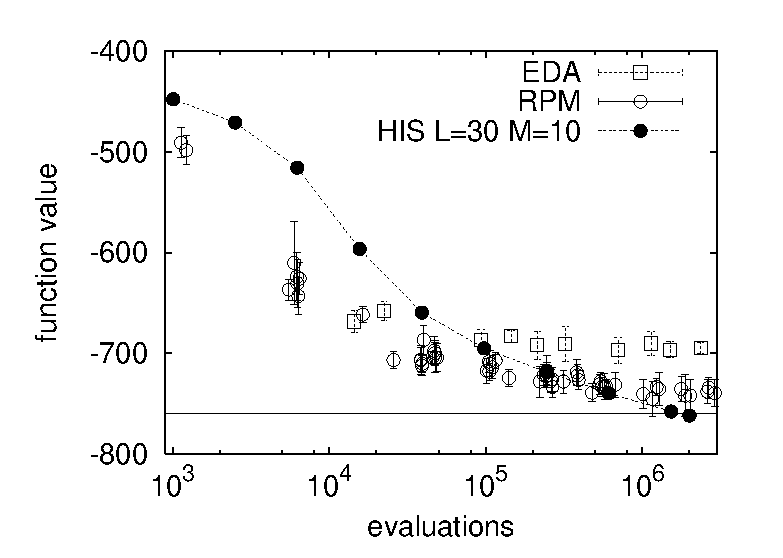
\includegraphics[width=\figlength\linewidth]{./data_aexp/2d_95.eps}}
\caption{2D Ising with $p(J^{-})=0.05$. 
The horizontal line is
 $y=800\times 0.95$ as a lower bound of the optimal solution. }
\label{result-2d-flust5}
\end{figure}
\begin{figure}[tbp]
\centerline{
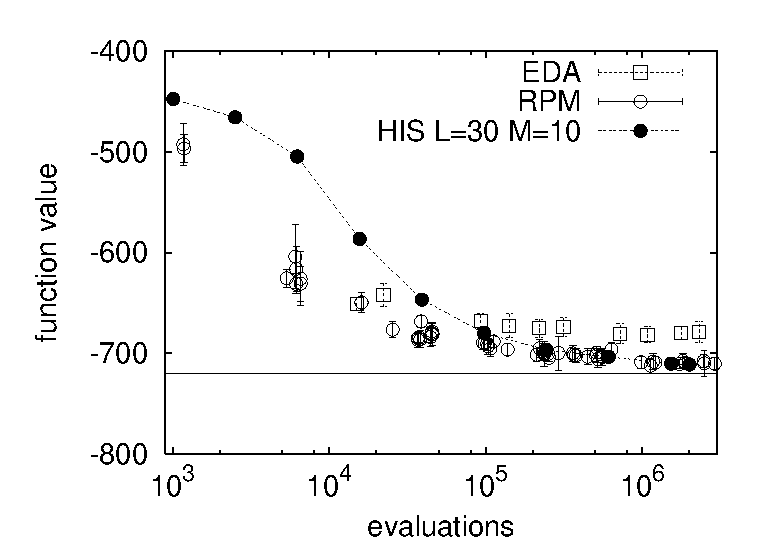
\includegraphics[width=\figlength\linewidth]{./data_aexp/2d_90.eps}}
\caption{2D Ising with $p(J^{-})=0.1$.
The horizontal line is
 $y=800\times 0.9$ as a lower bound of the optimal solution.}
\label{result-2d-flust10}
\end{figure}



\section{Experiments on Continuous Problems}
\subsection{Experimental Setup}
EDA, RPM and HIS are compared.
Their parameters are determined as follows:
\begin{itemize}
 \item EDA
       \begin{itemize}
	\item $M$: $500$, $1000$ or $3000$.
	\item $c$:  $0.3$.
       \end{itemize}
 \item RPM
       \begin{itemize}
	\item $M=N$: $50$, $100$ or $200$.
	\item $c$: $0.01$.      
       \end{itemize}
 \item HIS
       \begin{itemize}
	\item $M$: $10$ (in UG cases) or $100$ (in MG cases).
	\item $L$: $20$, $40$ or $60$.
       \end{itemize}
\end{itemize}

For probability models, two types of Gaussian distributions are
employed.
One is univariate Gaussian (UG), which means
we assume that each dimension is independent and, hence,
estimate only the diagonal elements of the covariance matrix.
Another is the normal multivariate Gaussian (MG).

The initialized region is $[-10,10]^d$.
Additionally,
we experiment the case where the initialized region is $[0,10]^d$
for Rastrigin function.
This setting is named shifted-Rastrigin (S-Rastrigin).
The number of dimensions is $10$.
For each setting, we perform ten independent runs.


\subsection{Results}
The number of successful trials in ten independent runs
are shown in Figs.  \ref{aexp-cont-best-eda}, \ref{aexp-cont-best-rpm}, 
and \ref{aexp-cont-best-his}.
The success means to find a solution with cost function
value less than $10^{-4}$.
The average and the standard deviation of the number of function evaluations until
convergence of EDA and RPM 
are shown in Figs. \ref{aexp-cont-eva-eda} and  \ref{aexp-cont-eva-rpm}.
On the other hand, Fig. \ref{aexp-cont-eva-his} shows the number of function evaluations
until finding global optima of HIS. Note that the HIS cases where
the global optima have not been found are ignored.
The optimization task of HIS is stopped if the number of function
evaluations become more than $10^7$.
Figures  \ref{aexp-cont-eva-eda}, \ref{aexp-cont-eva-rpm}, 
and \ref{aexp-cont-eva-his} show the average cost function value of the
obtained best solutions.


\begin{table}[tbp]
\centering
\caption{\aexpcontinuous EDA.}
\begin{tabular}{|l|r|r|r|r|}
\hline
 & \multicolumn{1}{c|}{$M$} & \multicolumn{1}{l|}{Rosenbrock} & \multicolumn{1}{l|}{Rastrigin} & \multicolumn{1}{l|}{S-Rastrigin} \\ \hline
 & 500 & 0 & 10 & 10 \\ \cline{2-5}
UG & 1000 & 0 & 10 & 10 \\ \cline{ 2- 5}
 & 3000 & 0 & 10 & 10 \\ \hline
 & 500 & 0 & 10 & 0 \\ \cline{ 2- 5}
MG & 1000 & 0 & 10 & 0 \\ \cline{ 2- 5}
 & 3000 & 0 & 10 & 0 \\ \hline
\end{tabular}
\label{aexp-cont-best-eda}
%\end{table}


%\begin{table}[tbp]
\centering
\caption{\aexpcontinuous RPM.}
\begin{tabular}{|l|r|r|r|}
\hline
 & \multicolumn{1}{l|}{$N=M$} & \multicolumn{1}{l|}{Rosenbrock} & \multicolumn{1}{l|}{Rastrigin} \\ \hline
 & 50 & 9 & 0 \\ \cline{ 2- 4}
UG & 100 & 10 & 0 \\ \cline{ 2- 4}
 & 200 & 10 & 1 \\ \hline
 & 50 & 10 & 0 \\ \cline{ 2- 4}
MG & 100 & 10 & 0 \\ \cline{ 2- 4}
 & 200 & 10 & 0 \\ \hline
\end{tabular}
\label{aexp-cont-best-rpm}
%\end{table}

%\begin{table}[tbp]
\centering
\caption{\aexpcontinuous HIS.}
\begin{tabular}{|l|r|r|r|r|}
\hline
 & \multicolumn{1}{l|}{$L$} & \multicolumn{1}{l|}{Rosenbrock} & \multicolumn{1}{l|}{Rastrigin} & \multicolumn{1}{l|}{S-Rastrigin} \\ \hline
 & 20 & 0 & 10 & 10 \\ \cline{2-5}
UG & 40 & 0 & 10 & 10 \\ \cline{ 2- 5}
 &  60 & 0 & 10 & 10 \\ \hline
 &  20& 10 & 5 & 2 \\ \cline{ 2- 5}
MG & 40 & 10 & 6 & 7 \\ \cline{ 2- 5}
 & 60 & 10 & 10 & 10 \\ \hline
\end{tabular}
\label{aexp-cont-best-his}
\end{table}

\begin{table}[tbp]
\centering
\caption{\aexpcontinuousnum EDA.}
\begin{tabular}{|lr|rr|rr|} \hline
\multicolumn{1}{|l|}{}&\multicolumn{1}{|c|}{M} & \multicolumn{2}{l|}{Rosenbrock} & \multicolumn{2}{l|}{Rastrigin} \\ \hline
\multicolumn{1}{|l|}{\multirow{3}{*}{UG}} & 500 & 1.36E+05 & ~~(1.38E+03) & 1.52E+05 & ~~(7.56E+03) \\ \cline{2-6}
\multicolumn{1}{|l|}{} & 1000 & 2.73E+05 & ~~(1.70E+03) & 2.98E+05 & ~~(4.84E+03) \\ \cline{2-6}
\multicolumn{1}{|l|}{} & 3000 & 8.21E+05 & ~~(3.60E+03) & 9.02E+05 & ~~(2.32E+04) \\ \hline
\multicolumn{1}{|l|}{\multirow{3}{*}{MG}} & 500 & 1.21E+05 & ~~(5.39E+03) & 1.44E+05 & ~~(1.75E+03) \\ \cline{2-6}
\multicolumn{1}{|l|}{} & 1000 & 2.38E+05 & ~~(1.76E+03) & 2.90E+05 & ~~(7.50E+03) \\ \cline{2-6}
\multicolumn{1}{|l|}{} & 3000 & 7.09E+05 & ~~(4.07E+03) & 8.99E+05 & ~~(8.57E+03) \\ \hline
\end{tabular}
\label{aexp-cont-eva-eda}
%\end{table} %


%\begin{table}[tbp]
\centering 
\caption{\aexpcontinuousnum EDA.}
\begin{tabular}{|lr|rr|rr|} \hline
\multicolumn{1}{|l|}{}&\multicolumn{1}{|c|}{M} & \multicolumn{2}{l|}{Rosenbrock} & \multicolumn{2}{l|}{Rastrigin} \\ \hline
\multicolumn{1}{|l|}{\multirow{3}{*}{UG}} & 500 & 8.30E+00 & ~~(2.41E-02) & 7.64E-05 & ~~(1.38E-05) \\ \cline{2-6}
\multicolumn{1}{|l|}{} & 1000 & 8.28E+00 & ~~(1.50E-02) & 7.38E-05 & ~~(9.15E-06) \\ \cline{2-6}
\multicolumn{1}{|l|}{} & 3000 & 8.25E+00 & ~~(4.27E-02) & 8.22E-05 & ~~(1.07E-05) \\ \hline
\multicolumn{1}{|l|}{\multirow{3}{*}{MG}} & 500 & 7.89E+00 & ~~(1.59E-01) & 8.30E-05 & ~~(1.95E-05) \\ \cline{2-6}
\multicolumn{1}{|l|}{} & 1000 & 7.98E+00 & ~~(9.23E-02) & 7.88E-05 & ~~(1.20E-05) \\ \cline{2-6}
\multicolumn{1}{|l|}{} & 3000 & 7.91E+00 & ~~(6.77E-02) & 7.36E-05 & ~~(1.22E-05) \\ \hline
\end{tabular}
\label{aexp-cont-val-eda}
%\end{table} %


%\begin{table}[tbp]
\centering 
\caption{The average cost function value of the obtained solutions and the average number of function
 evaluations  of EDA for S-Rastrigin.}
\begin{tabular}{|lr|rr|rr|} \hline
\multicolumn{1}{|l|}{}&\multicolumn{1}{|c|}{M} & \multicolumn{2}{l|}{Value} & \multicolumn{2}{l|}{Num. of Evaluations} \\ \hline
\multicolumn{1}{|l|}{\multirow{3}{*}{UG}} & 500 & 8.36E-05 & ~~(1.44E-05) & 1.79E+05 & ~~(9.67E+03) \\ \cline{2-6}
\multicolumn{1}{|l|}{} & 1000 & 7.38E-05 & ~~(1.51E-05) & 3.39E+05 & ~~(1.51E+04) \\ \cline{2-6}
\multicolumn{1}{|l|}{} & 3000 & 8.48E-05 & ~~(1.01E-05) & 9.98E+05 & ~~(1.76E+04) \\ \hline
\multicolumn{1}{|l|}{\multirow{3}{*}{MG}} & 500 & 5.16E+01 & ~~(6.93E+00) & 4.85E+06 & ~~(4.72E+06) \\ \cline{2-6}
\multicolumn{1}{|l|}{} & 1000 & 4.63E+01 & ~~(4.98E+00) & 3.28E+06 & ~~(4.40E+06) \\ \cline{2-6}
\multicolumn{1}{|l|}{} & 3000 & 3.93E+01 & ~~(8.03E-01) & 1.09E+06 & ~~(6.35E+04) \\ \hline
\end{tabular}
\label{aexp-cont-srast-eda}
\end{table} %


\begin{table}[tbp]
\centering 
\caption{\aexpcontinuousnum RPM.}
\begin{tabular}{|lr|rr|rr|} \hline
\multicolumn{1}{|l|}{}&\multicolumn{1}{|c|}{M=N} & \multicolumn{2}{l|}{Rosenbrock} & \multicolumn{2}{l|}{Rastrigin} \\ \hline
\multicolumn{1}{|l|}{\multirow{3}{*}{UG}} & 50 & 7.93E+05 & ~~(5.31E+05) & 4.72E+05 & ~~(2.53E+05) \\ \cline{2-6}
\multicolumn{1}{|l|}{} & 100 & 1.71E+06 & ~~(6.61E+04) & 2.92E+06 & ~~(2.07E+06) \\ \cline{2-6}
\multicolumn{1}{|l|}{} & 200 & 3.88E+06 & ~~(1.56E+05) & 1.60E+07 & ~~(2.56E+05) \\ \hline
\multicolumn{1}{|l|}{\multirow{3}{*}{MG}} & 50 & 3.06E+05 & ~~(7.69E+03) & 3.49E+05 & ~~(9.27E+04) \\ \cline{2-6}
\multicolumn{1}{|l|}{} & 100 & 1.46E+06 & ~~(3.13E+04) & 2.71E+06 & ~~(5.32E+04) \\ \cline{2-6}
\multicolumn{1}{|l|}{} & 200 & 4.00E+06 & ~~(1.04E+05) & 1.10E+07 & ~~(2.50E+05) \\ \hline
\end{tabular}
\label{aexp-cont-eva-rpm}
%\end{table} %


%\begin{table}[tbp]
\centering 
\caption{\aexpcontinuousval RPM.}
\begin{tabular}{|lr|rr|rr|} \hline
\multicolumn{1}{|l|}{}&\multicolumn{1}{|c|}{M=N} & \multicolumn{2}{l|}{Rosenbrock} & \multicolumn{2}{l|}{Rastrigin} \\ \hline
\multicolumn{1}{|l|}{\multirow{3}{*}{UG}} & 50 & 2.95E+02 & ~~(8.84E+02) & 1.48E+01 & ~~(1.39E+01) \\ \cline{2-6}
\multicolumn{1}{|l|}{} & 100 & 2.31E-04 & ~~(2.70E-05) & 1.67E+01 & ~~(1.63E+01) \\ \cline{2-6}
\multicolumn{1}{|l|}{} & 200 & 1.37E-04 & ~~(1.68E-05) & 2.59E+00 & ~~(1.95E+00) \\ \hline
\multicolumn{1}{|l|}{\multirow{3}{*}{MG}} & 50 & 7.94E-05 & ~~(1.48E-05) & 1.03E+01 & ~~(9.19E+00) \\ \cline{2-6}
\multicolumn{1}{|l|}{} & 100 & 8.45E-05 & ~~(1.06E-05) & 1.09E+01 & ~~(4.36E+00) \\ \cline{2-6}
\multicolumn{1}{|l|}{} & 200 & 7.84E-05 & ~~(1.57E-05) & 6.57E+00 & ~~(3.12E+00) \\ \hline
\end{tabular}
\label{aexp-cont-val-rpm}
\end{table} %


\begin{table}[tbp]
\centering 
\caption{\aexpcontinuousnum HIS.}
\begin{tabular}{|lr|rr|rr|} \hline
\multicolumn{1}{|l|}{}&\multicolumn{1}{|c|}{L} & \multicolumn{2}{l|}{Rosenbrock} & \multicolumn{2}{l|}{Rastrigin} \\ \hline
\multicolumn{1}{|l|}{\multirow{3}{*}{UG}} & 20 & 1.00E+07 & ~~(0.00E+00) & 2.01E+05 & ~~(5.88E+04) \\ \cline{2-6}
\multicolumn{1}{|l|}{} & 40 & 1.00E+07 & ~~(0.00E+00) & 4.23E+05 & ~~(1.84E+05) \\ \cline{2-6}
\multicolumn{1}{|l|}{} & 60 & 1.00E+07 & ~~(0.00E+00) & 5.94E+05 & ~~(1.75E+05) \\ \hline
\multicolumn{1}{|l|}{\multirow{3}{*}{MG}} & 20 & 2.74E+05 & ~~(2.64E+04) & 2.40E+06 & ~~(3.08E+06) \\ \cline{2-6}
\multicolumn{1}{|l|}{} & 40 & 5.09E+05 & ~~(3.56E+04) & 2.65E+06 & ~~(1.77E+06) \\ \cline{2-6}
\multicolumn{1}{|l|}{} & 60 & 7.91E+05 & ~~(6.64E+04) & 2.23E+06 & ~~(4.28E+05) \\ \hline
\end{tabular}
\label{aexp-cont-eva-his}
%\end{table} %


%\begin{table}[tbp]
\centering 
\caption{\aexpcontinuousval HIS.}
\begin{tabular}{|lr|rr|rr|} \hline
\multicolumn{1}{|l|}{}&\multicolumn{1}{|c|}{L} & \multicolumn{2}{l|}{Rosenbrock} & \multicolumn{2}{l|}{Rastrigin} \\ \hline
\multicolumn{1}{|l|}{\multirow{3}{*}{UG}} & 20 & 4.13E+00 & ~~(8.12E-02) & 8.80E-05 & ~~(1.47E-05) \\ \cline{2-6}
\multicolumn{1}{|l|}{} & 40 & 4.07E+00 & ~~(5.05E-01) & 9.05E-05 & ~~(8.98E-06) \\ \cline{2-6}
\multicolumn{1}{|l|}{} & 60 & 7.02E+00 & ~~(6.42E-01) & 8.47E-05 & ~~(1.53E-05) \\ \hline
\multicolumn{1}{|l|}{\multirow{3}{*}{MG}} & 20 & 6.64E-05 & ~~(1.61E-05) & 5.97E-01 & ~~(6.60E-01) \\ \cline{2-6}
\multicolumn{1}{|l|}{} & 40 & 7.21E-05 & ~~(2.24E-05) & 6.97E-01 & ~~(8.95E-01) \\ \cline{2-6}
\multicolumn{1}{|l|}{} & 60 & 7.89E-05 & ~~(1.37E-05) & 8.33E-05 & ~~(1.83E-05) \\ \hline
\end{tabular}
\label{aexp-cont-val-his}
%\end{table} %


%\begin{table}[tbp]
\centering 
\caption{The average cost function value of the obtained solutions and the average number of function
 evaluations  of HIS for S-Rastrigin.}
\begin{tabular}{|lr|rr|rr|} \hline
\multicolumn{1}{|l|}{}&\multicolumn{1}{|c|}{L} & \multicolumn{2}{l|}{Value} & \multicolumn{2}{l|}{Num. of Evaluations} \\ \hline
\multicolumn{1}{|l|}{\multirow{3}{*}{UG}} & 20 & 7.35E-05 & ~~(2.66E-05) & 1.93E+05 & ~~(9.52E+04) \\ \cline{2-6}
\multicolumn{1}{|l|}{} & 40 & 8.87E-05 & ~~(1.17E-05) & 4.15E+05 & ~~(1.45E+05) \\ \cline{2-6}
\multicolumn{1}{|l|}{} & 60 & 8.96E-05 & ~~(1.12E-05) & 5.40E+05 & ~~(1.47E+05) \\ \hline
\multicolumn{1}{|l|}{\multirow{3}{*}{MG}} & 20 & 1.49E+00 & ~~(1.20E+00) & 2.60E+05 & ~~(3.90E+06) \\ \cline{2-6}
\multicolumn{1}{|l|}{} & 40 & 3.98E-01 & ~~(6.60E-01) & 2.53E+06 & ~~(4.16E+06) \\ \cline{2-6}
\multicolumn{1}{|l|}{} & 60 & 8.76E-05 & ~~(1.10E-05) & 1.96E+06 & ~~(9.47E+05) \\ \hline
\end{tabular}
\label{aexp-cont-srast-his}
\end{table}


%%%%%%%%%%%%%%%%%%%%%%%%%%%%%%%%%%%%%%%%%%%%%%%%%%%%%%%%%%%%%%%%%
\begin{comment}
\begin{table}[tbp]
\centering
\caption{The Number of Successful Trials Finding Global Optima with Univariate Gaussian.}
\begin{tabular}{|c|r|r|r|}
\hline
& \multicolumn{1}{c|}{EDA} & \multicolumn{1}{c|}{RPM} & \multicolumn{1}{c|}{HIS} \\ \hline
Rosenbrock & 0 & 10 & 0 \\ \hline
Rastrigin & 10 & 0 & 10 \\ \hline
S-Rastrigin & 10 & 0 & 10 \\ \hline
\end{tabular}
\label{aexp-ugauss}
\end{table}

\begin{table}[tbp]
\centering
\caption{The Number of Successful Traials Finding Global Optima with
 Multivariate Gaussian.}
\begin{tabular}{|c|r|r|r|}
\hline
& \multicolumn{1}{c|}{EDA} & \multicolumn{1}{c|}{RPM} & \multicolumn{1}{c|}{HIS} \\ \hline
Rosenbrock & 0 & 10 & 10 \\ \hline
Rastrigin & 10 & 0 & 3 \\ \hline
S-Rastrigin & 0 & 0 & 3 \\ \hline
\end{tabular}
\label{aexp-mgauss}
\end{table}

\begin{table}[tbp]
\footnotesize
\centering
\caption{The Number of Function Evalutions with Univariate Gaussian.}
\begin{tabular}{|c|rr|rr|rr|}
\hline
 & \multicolumn{2}{c|}{EDA}  & \multicolumn{2}{c|}{RPM} &
 \multicolumn{2}{c|}{HIS} \\ \hline 
Rosenbrock & 820800 & (2749.55) & 1188310 & (53425.15) & 1000011 & (0) \\ \hline
Rastrigin & 891600 & (8979.98) & 1119080 & (616628.28) & 1828426.1 & (2481839.34) \\ \hline
S-Rastrigin & 985800 & (19218.74) & 1416100 & (429720.21) & 133036.9 & (116780.09) \\ \hline
\end{tabular}
\label{aexp-ugauss-eva}
\end{table}

\begin{table}[tbp]
\footnotesize
\centering
\caption{The Number of Function Evaluations with Multivariate Gaussian.}
\begin{tabular}{|c|rr|rr|rr|}
\hline
& \multicolumn{2}{c|}{EDA} &   \multicolumn{2}{c|}{RPM} &
 \multicolumn{2}{c|}{HIS}  \\ \hline
Rosenbrock & 719700 & (8100) & 644750 & (16173.95) & 228130 & (21290.47) \\ \hline
Rastrigin & 985800 & (11864.23) & 989410 & (29525.46) & 405110 & (146323) \\ \hline
S-Rastrigin & 1144500 & (136802.96) & 929570 & (142713.99) & 418500 & (128180.5) \\ \hline
\end{tabular}
\label{aexp-mgauss-eva}
\end{table}
\end{comment}


The results show that
EDA cannot find the optima in Rosenbrock function where as
can find the optima  in Rastrigin function.
In S-Rastrigin, EDA using MG cannot find the optimal solution where as
EDA using UG can find.
When using UG, only RPM can find the optima in Rosenbrock function.
On the other hand, Rastrigin function is too difficult for RPM 
HIS can find the optima both Rastrigin and S-Rastrigin if
the number of the layers is sufficiently large.
In general results depend on the number of function evaluations, that is, 
the convergence speed.
The difference of the number of function evaluations among the settings
is not significantly large in log-scale.

\section{Discussion}

\subsection{Robustness against Frustration}
The frustration has an effect on the instability.
Through experiments, 
it seems that 
the frustration does not cause serious problems
because the cost function value of the obtained solution is 
near the estimated optimal cost function value.
The instability can be removed through 
the annealing process.


\subsection{Difficulty in 2D Ising Model}
The difference among the thee method is reduced by adding the frustration.
This can be explained by the 
size of the clusters.
Basically, the optimization process of EAPM for 2D Ising consists of
three phases.
The first phase is the transition from random to some clusters.
A cluster means 
a set of connected variables which have the same value.
In the second phase, the clusters are merged.
In the third phase, two clusters remains and consequently one has to be
eliminated
in order to obtain the optimal solution.
Actually, to eliminate a big cluster is quite difficult for EAPM.
However, the frustration breaks the large clusters.


\subsection{RPM: Robustness against Model Error}
For Rosenbrock function,
RPM can find the global optima in spite of using 
the inappropriate probability model, that is, UG,
whereas HIS cannot in the same condition.
This shows the robustness against the model error,
which means the difference 
between the target distribution and the probability model.
RPM can store a part of the historical samples and
this mechanism do not depend on the probability model in theory.



\subsection{HIS: Robustness against Local Optima}
HIS works well for Rastrigin,
whereas RPM do not.
The reason would be the presence of the local optima.
The number of local optima around the global optima is
at least $3^{d}-1$ and RPM drops into one of them.
In practice $d=5$, RPM can find the global optima.

The reason of HIS finding the global optima is
preserving the best probability model.
This can be understood as preserving the best obtained samples,
whereas RPM may discard the best samples in order to remove the bias.
Note that HIS removes the bias according to importance sampling
with different manner from RPM.


\subsection{Estimation Bias in EDA}
In cases using MG,
EDA seems to be effective for Rastrigin function.
However, we have to note the bias of EDA.
In importance sampling, EDA assumes the following:
\begin{equation}
 \frac{q_{t+1}(x)}{p_t(x)} \log p(x|w) \simeq 
 \frac{q_{t+1}(x)}{q_t(x)} \log p(x|w),
\end{equation} 
where target distributions are supposed to be 
partially uniform distributions.
The simple aspect is the assumption of
\begin{equation}
 q_t(x)=p_t(x).
\end{equation}
This is the assumption that
 the statistical estimation is completely successful.
This has an effect on the variance reduction but
we estimate the following distribution:
\begin{equation}
 q^{bias}_{t+1}(x)=\frac{p_t(x)}{q_t(x)}q_{t+1}(x).
\end{equation}
This can be the reason of the failure 
in Rosenbrock function and S-Rastrigin function
with MG.


\begin{table}
\centering
\begin{tabular}{|c|c|c|c|}
\hline 
&  Model Error & Local Optima & Removing Bias \\
\hline
EDA & ? & ? & Bad \\
\hline
RPM & Good & Bad & Good \\
\hline
HIS & Bad & Good & Good \\
\hline
\end{tabular}
\end{table}



\section{Summary}
This chapter provides experimental results to investigate
additional properties of EDA, RPM and HIS.
The experiments have revealed that
RPM has the robustness against the model error and
HIS has the robustness against local optima and.
